\documentclass{standalone}
\usepackage[T1]{fontenc}
\usepackage[utf8]{inputenc}
\usepackage[usenames,dvipsnames]{xcolor}
\usepackage{tikz}
\usetikzlibrary{plotmarks}
\usetikzlibrary{shapes,snakes,arrows}
\begin{document}
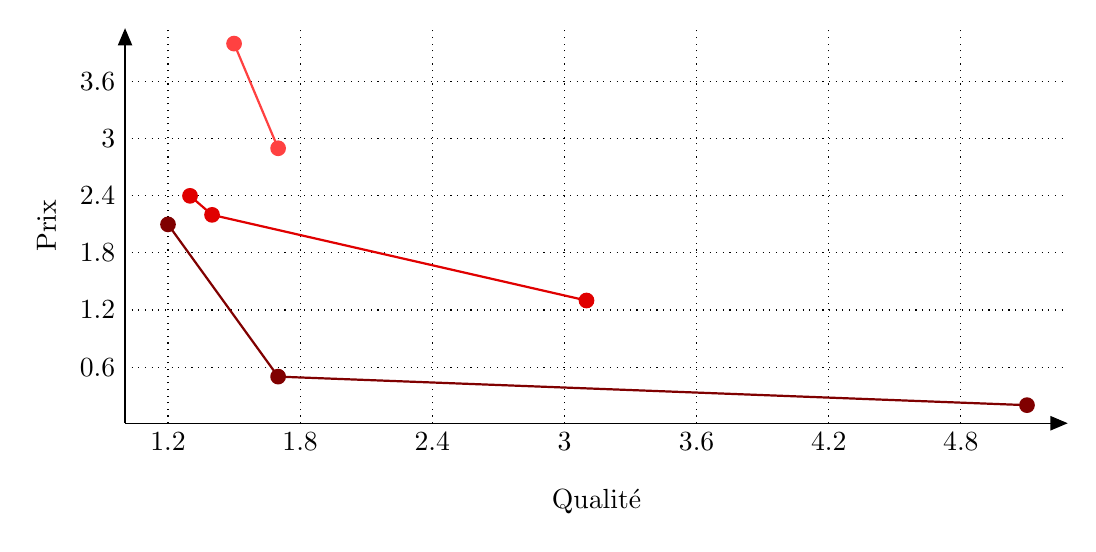
\begin{tikzpicture}[xscale=2.7972,yscale=1.20839]
\draw[xstep=0.6,ystep=0.6,thin,dotted,color=Black] (1.005,0.01) grid (5.28486,4.16156);
\begin{scope}
  \clip (1.005,0.01) rectangle (5.28486,4.16156);
  \definecolor{pLineColor}{RGB}{128,0,0}
  \definecolor{pPointColor}{RGB}{128,0,0}
  \draw[thick,color=pPointColor] (1.2,2.1) node[color=pPointColor,fill=pPointColor, circle, inner sep = 0pt, minimum size=2mm] {} -- (1.7,0.5) node[color=pPointColor,fill=pPointColor, circle, inner sep = 0pt, minimum size=2mm] {} -- (5.1,0.2) node[color=pPointColor,fill=pPointColor, circle, inner sep = 0pt, minimum size=2mm] {};
  \definecolor{pLineColor}{RGB}{224,0,0}
  \definecolor{pPointColor}{RGB}{224,0,0}
  \draw[thick,color=pPointColor] (1.3,2.4) node[color=pPointColor,fill=pPointColor, circle, inner sep = 0pt, minimum size=2mm] {} -- (1.4,2.2) node[color=pPointColor,fill=pPointColor, circle, inner sep = 0pt, minimum size=2mm] {} -- (3.1,1.3) node[color=pPointColor,fill=pPointColor, circle, inner sep = 0pt, minimum size=2mm] {};
  \definecolor{pLineColor}{RGB}{255,65,65}
  \definecolor{pPointColor}{RGB}{255,65,65}
  \draw[thick,color=pPointColor] (1.5,4) node[color=pPointColor,fill=pPointColor, circle, inner sep = 0pt, minimum size=2mm] {} -- (1.7,2.9) node[color=pPointColor,fill=pPointColor, circle, inner sep = 0pt, minimum size=2mm] {};
\end{scope}
\draw[->,>=triangle 45] (1.005,0.01) -- coordinate (x axis mid) (5.28486,0.01);
\node[below=1cm,anchor=center] at (x axis mid) {Qualité};
\foreach \x in {1.2,1.8,2.4,3,3.6,4.2,4.8}
  \draw (\x,0.01) -- (\x,0.01) node[anchor=north] {\x};
\draw[->,>=triangle 45] (1.005,0.01) -- coordinate (y axis mid) (1.005,4.16156);
\node[left=1cm,rotate=90,anchor=center] at (y axis mid) {Prix};
\foreach \y in {0.6,1.2,1.8,2.4,3,3.6}
  \draw (1.005,\y) -- (1.005,\y) node[anchor=east] {\y};
\end{tikzpicture}
\end{document}
